%%%%%%%%%%%%%%%%%%%%%%%%%%%%%%%%%%%%%%%%%%%%%%%%%
%
%     Chapter 6
%
%%%%%%%%%%%%%%%%%%%%%%%%%%%%%%%%%%%%%%%%%%%%%%%%

\chapter{Performance Evaluation}
\label{six}

In this chapter, we focus on the performance evaluation to show that our LLVM backend could not only match performance with the hand-written library, but also provide a better chance to optimize according to the specific target. We would first validate our vector of $i2^k$ approaches, and then present the performance of some Parabix applications.

\section{Vector of $i2^k$ Performance}
In Chapter~\ref{four}, we present different approaches to lower $i1$, $i2$, $i4$ and some $i8$ operations within one SIMD register. In this section, we would validate our approaches by showing the improved runtime performance. We would use two major measurement: the elaborated micro benchmarks and the SelectionDAG size. Some of the vector type like $i2$ cannot get compiled correctly on LLVM 3.5, so we resort to compare the size of the generated SelectionDAG, assuming that the larger the DAG is, the more complexed code would be generated.

\subsection{Methodology}

Testing small pieces of critical code can be tricky, since the testing overhead can easily overwhelm the critical code and make the result meaningless. Dr. Agner Fog provides a test program which uses the Time Stamp Counter for clock cycles and Performance Monitor Counters for instruction count and other related events \cite{agner_testp}. We pick the reciprocal throughput as our measurement and it is measured with a sequence of same instructions where subsequent instructions are independent of the previous ones. In Dr. Fog's instruction table, he noted that a typical length of the sequence is 100 instructions of the same type and this sequence should be repeated in a loop if a larger number of instructions is desired.

We did one simple experiment with SIMD XOR ($xorps$) to validate this program. Refer to Figure~\ref{figure:testp_xor}, we measured the performance of executing different number of XOR instructions; they are organized into one for loop and we have checked the assembly code to make sure the XOR operations are not optimized away.

\begin{figure}[ht!]
\centering
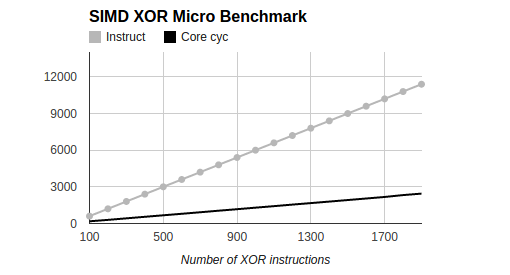
\includegraphics[width=140mm]{draw/testp_xor.png}
\caption[Test Performance with XOR]{Test performance with XOR\@.}
\label{figure:testp_xor}
\end{figure}

From the figure, we can see the instructions count and CPU cycles grows linearly with the number of XOR instructions. So we can conclude that Dr. Fog's test program can be used to compare two pieces of critical code: the one with more measured CPU cycles is more complex and have more instructions. Note that from the figure, it seems the throughput of $xorps$ is 4, which is different from Intel's document (3 in document). We found this may be related to the compiler optimization on the loop; when we flattened the loop we got the throughput around 2 to 3. In order to eliminate this undesired effect, we would flatten the test code in the following sections.

In the following sections, we would write micro benchmarks with Agner Fog's test program and compare reciprocal throughput between different implementation. Our test machine is X86 64-bit Ubuntu with Intel Haswell, and the detailed configuration can be found in Table~\ref{table:hardware_config}. In order to inline pure IR functions (instead of a function call into one object file), we compile all the test code into LLVM bitcode (binary form of LLVM IR) and then link / optimize them together.

\begin{table}[h]
\centering
\begin{tabular}{|c|c|}
\hline
CPU Name       & Intel(R) Core(TM) i5-4570 CPU \\ \hline
CPU MHz        & 3200                          \\ \hline
FPU            & Yes                           \\ \hline
CPU(s) enabled & 4 cores                       \\ \hline
L1 Cache       & 32 KB D + 32KB I              \\ \hline
L2 Cache       & 256 KB                        \\ \hline
L3 Cache       & 6 MB                          \\ \hline
Memory         & 8GB                           \\ \hline
\end{tabular}
\caption{Hardware Configuration}
\label{table:hardware_config}
\end{table}

\begin{table}[h]
\centering
\begin{tabular}{|c|c|}
\hline
Operating System & Ubuntu (Linux X86-64)         \\ \hline
Compiler         & Clang 3.5-1ubuntu1, GCC 4.8.2 \\ \hline
LLVM             & LLVM 3.5                      \\ \hline
File System      & Ext4                          \\ \hline
\end{tabular}
\caption{Software Configuration}
\label{table:software_config}
\end{table}

\subsection{Performance Against IDISA}
We compare our lowering on pure IR function with IDISA+ Library \cite{hua_idisa} which is written in C++. To test each operation, we generate a sequence of 500 such operations where none them has to wait for the previous one. 100 operations seems not long enough for a stable result. The performance comparison is listed in Figure~\ref{figure:vector_perf_idisa}. We can see for $i1$ and $i4$ vectors, IR library has the similar performance with IDISA but it performs better with $i2$ vectors, especially on integer comparison.

The underlying logic for both libraries is the same, but it is implemented in different level. For IDISA library, {\tt simd<2>::ugt} got inline-extended immediately by the compiler front end and its semantics of integer comparison lost ever after, while in the IR library, for the whole life cycle before the instruction selection, {\tt ugt\_2} keeps its semantics and this may help the compiler to optimize. The expansion of {\tt ugt\_2} is delayed until the instruction selection phase, right before machine code generation. We checked that IDISA function {\tt simd<2>::ugt} and IR function {\tt ugt\_2} (whose underlying code is just \verb|icmp ugt <64 x i2> %a, %b|) generated different assembly code.

However, the delay in expansion is not always good. Take multiplication on $i2$ vector for an example, we can see our IR library has slightly better performance on it. But if we write our instructions sequence with a loop, IDISA library would win. Loop optimization should be responsible for this difference and we did observe some kind of hoisting in the assembly code. Early expansion in IDISA also provides more optimization opportunity to the compiler front end.

\begin{figure}[ht!]
\centering
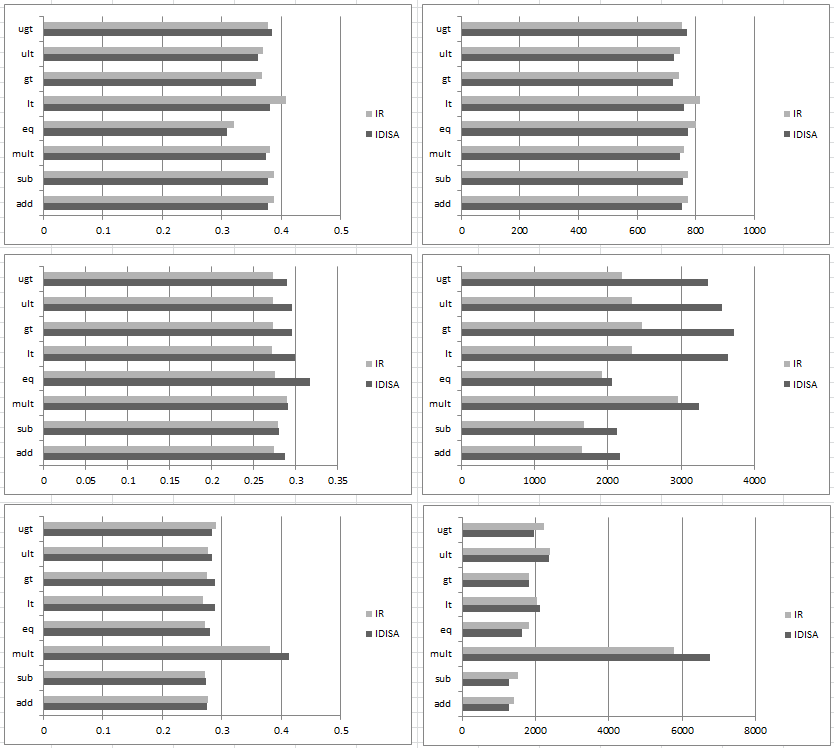
\includegraphics[width=140mm]{draw/vector_idisa_perf.png}
\caption[Performance Against IDISA Library]{Performance against IDISA Library. The left column is the reciprocal throughput and the right column is the core CPU cycles.}
\label{figure:vector_perf_idisa}
\end{figure}

\subsection{Performance Against LLVM}
We compare our lowering with native LLVM\@. LLVM could not handle $i2$, $i4$ vectors and handle $i1$ vectors slowly. Detailed performance data can be found in Table~\ref{table:vector_perf_LLVM}. We can see that our approach fills the gap of LLVM type system.

\begin{table}[h]
\centering
\begin{tabular}{|c|c|c|c|}
\hline
     & $i1$ & $i2$ & $i4$ \\ \hline
add  & 302  & X    & X    \\ \hline
sub  & 310  & X    & X    \\ \hline
mult & X    & X    & X    \\ \hline
eq   & 273  & X    & X    \\ \hline
lt   & X    & X    & X    \\ \hline
gt   & X    & X    & X    \\ \hline
ult  & 349  & X    & X    \\ \hline
ugt  & 290  & X    & X    \\ \hline
\end{tabular}
\caption[LLVM Native Support for $i1$, $i2$, $i4$ Vectors]{LLVM native support of $i1$, $i2$, $i4$ vectors. X means compile error or compile too slowly (longer than 30s), the rest number means the ratio of CPU cycles against our lowering: add takes 302 times of the cycles that our lowering needs.}
\label{table:vector_perf_LLVM}
\end{table}

\section{Parabix Critical Operations}
In this section, we evaluate our work by replacing Parabix critical operations with IR library. We choose transposition and reverse transposition as two representative operations and measure performance in two Parabix applications: XML validator and UTF-8 to UTF-16 transcoder. Note that we did not rewrite the whole application with an IR library, part of the application is still IDISA but some critical operation is replaced.

\begin{table}[h]
\centering
\begin{tabular}{|c|c|c|c|c|c|}
\hline
        & dew.xml  &  jaw.xml  &  roads-2.gml  &  po.xml  & soap.xml¬ \\\hline
xmlwf0   &  3.93   &    4.364   &   4.553   &   4.891   &   5.18 \\ \hline
xmlwf0 on Haswell   &  3.929   &   4.363   &   4.554   &   4.876   &   5.178 \\ \hline

xmlwf1   &  3.929   &   4.371   &   4.566   &   4.861   &   5.186 \\ \hline
xmlwf1 on Haswell &   3.566   &   3.978   &   4.163   &   4.451   &   4.787 \\ \hline
\end{tabular}
\caption[Performance Comparison of XML Validator (xmlwf)]{Performance comparison of XML validator (xmlwf). In the table, xmlwf0 is implemented with full IDISA library and xmlwf1 is a copy of xmlwf0 with the transposition replaced.}
\label{table:xmlwf_perf}
\end{table}

Table~\ref{table:xmlwf_perf} shows the performance of the XML Validator. The only difference of xmlwf0 and xmlwf1 is their transposition code, and the one in xmlwf1 is written in pure IR with the byte-pack algorithm. We can see xmlwf0 and xmlwf1 share almost identical performance and it is not for free. LLVM 3.5 cannot handle packing on 16-bit field width very well and we custom lower the shufflevector and generate PACKUS instruction for X86.

Another interesting observation is, when we re-compiled the same code on the Intel Haswell platform, we got almost no improvement for xmlwf0, since the IDISA library is for SSE2 and it is written with SSE2 intrinsics; but we got a slightly better performance for xmlwf1, because LLVM backend knows other instruction set like SSE3, SSE4 is available on this platform and thus generating better native code.

\section{Long Stream Addition / Shift}

